\documentclass[DIN, pagenumber=false, fontsize=11pt, parskip=half]{scrartcl}

\usepackage{amsmath}
\usepackage{amsfonts}
\usepackage{amssymb}
\usepackage{enumitem}
\usepackage[utf8]{inputenc} 
\usepackage[ngerman]{babel} 
\usepackage[T1]{fontenc} 
\usepackage{pgfplots}
\usepackage{xcolor}
\usepackage{listings}
\usepackage{float}
\usepackage{graphicx}
\usepackage{booktabs}
\usepackage{tkz-euclide}
\usepackage{svg}

\definecolor{mygreen}{RGB}{28,172,0} % color values Red, Green, Blue
\definecolor{mylilas}{RGB}{170,55,241}

\tikzstyle{neuron}=[circle,fill=black!25,minimum size=30pt,inner sep=0pt]

\lstset{language=Matlab,%
    %basicstyle=\color{red},
    breaklines=true,%
    morekeywords={matlab2tikz},
    keywordstyle=\color{blue},%
    morekeywords=[2]{1}, keywordstyle=[2]{\color{black}},
    identifierstyle=\color{black},%
    stringstyle=\color{mylilas},
    commentstyle=\color{mygreen},%
    showstringspaces=false,%without this there will be a symbol in the places where there is a space
    numbers=left,%
    numberstyle={\tiny \color{black}},% size of the numbers
    numbersep=9pt, % this defines how far the numbers are from the text
    emph=[1]{for,end,break},emphstyle=[1]\color{red}, %some words to emphasise
    %emph=[2]{word1,word2}, emphstyle=[2]{style},    
}

\title{Einführung in die Neuroinformatik}
\author{Tim Luchterhand, Paul Nykiel (Gruppe P)}

\begin{document}
    \maketitle
    \section{Learning Slowdown}
    \subsection{}
    \begin{enumerate}[label=(\alph*)]
        \item 
            \begin{eqnarray*}
                w_2 &=& 0.6 \\
                b_2 &=& 0.9 \\
                T &=& 0 \\
                \Rightarrow \frac{\partial E}{\partial b_2} (w,b) &=& -2 \left( 0- \frac{1}{1+e^{-1.5}} \right) \frac{1}{1+e^{-1.5}} \left( 1 -\frac{1}{1+e^{-1.5}}\right) \\
                &\approx& 0.24
            \end{eqnarray*}
        \item 
            \begin{eqnarray*}
                w_2 &=& 2 \\
                b_2 &=& 2 \\
                T &=& 0 \\
                \Rightarrow \frac{\partial E}{\partial b_2} (w,b) &=& -2 \left( 0- \frac{1}{1+e^{-4}} \right) \frac{1}{1+e^{-4}} \left( 1 -\frac{1}{1+e^{-4}}\right) \\
                &\approx& 0.035
            \end{eqnarray*}
        \item Der Gradient ist sehr klein, wodurch jede Epoche nur minimalen Lernfortschrittt bringt. Problematisch ist hierbei die Ableitung der Sigmoid-Funktion, da $f'(x) \in \left[0, \frac{1}{4}\right]\ \forall x \in \mathbb{R}$, und verschwindet für betragsmäßig große $x$.
    \end{enumerate}

    \subsection{}
    \begin{enumerate}[label=(\alph*)]
        \item 
            \begin{eqnarray*}
                \frac{\partial E}{\partial b_1} &=& 2 (T-y_2) \cdot (-1) \cdot \frac{\partial y_2}{\partial b_1} \\
                &=& -2 (T-y_2) \cdot \frac{\partial}{\partial b_1} f(w_2 \cdot f(w_1 \cdot x + b_1) + b_2) \\
                &=& -2 (T-y_2) \cdot f'(w_2 \cdot f(w_1 \cdot x + b_1) + b_2) \cdot w_2 \cdot f'(w_1 \cdot x + b_1) \\
                &=& -2 (T-y_2) \cdot f'(u_2) \cdot w_2 \cdot f'(u_1)
            \end{eqnarray*}
            Pro weiterer Netzwerkschicht kommen weitere $f'$-Terme hinzu die wiederrum $\in \left[0, \frac{1}{4}\right]$ sind. Dadurch wird der Gradient tendentiell noch kleiner und das Lernen verlangsamt sich zusätzlich zu Neuronen näher zur Eingangsschicht.
        \item Wie in (a) bereits erläutert, verschlimmern weitere Schichten das Problem.
        \item In jeder Epoche werden die Gewichte und der Bias nur marginal angepasst wodurch der Gradientenabstieg sehr langsam erfolgt.
    \end{enumerate}

    \subsection{}
    \begin{enumerate}[label=(\alph*)]
        \item 
            \begin{eqnarray*}
                x &=& 1 \\
                T &=& 0 \\
                w_1 &=& 100 \\
                b_1 &=& -100 \\
                w_2 &=& 100 \\
                b_2 &=& -50 \\
                u_1 &=& 100 - 100 = 0 \\
                y_1 &=& f(u_1) = \frac{1}{2} \\
                u_2 &=& 100 \cdot y_1 - 50 = 0 \\
                y_2 &=& f(u_2) = \frac{1}{2} \\
                \frac{\partial E}{\partial b_2} &=& 2 \cdot y_2 \cdot f'(u_2) ) = \frac{1}{4} \\
                \frac{\partial E}{\partial b_1} &=& \frac{\partial E}{\partial b_2} \cdot 25 = \frac{25}{4} 
            \end{eqnarray*}
        \item 
            Der Gradient der aktuellen Schicht setzt sich aus dem Gradienten der Nachfolgenden Schicht multipliziert mit einem Faktor $\gg1$. Dadurch werden die Gradienten in den Schichten nah am Eingang extrem groß.
        \item Ein zu großer Gradient kann dazu führen, dass Minima übersprungen werden wodurch der Lernprozess oszilliert und sich das Lernen in die Länge zieht.
    \end{enumerate}

    \subsection{}
    Bei der Cross-Corelation-Funktion tritt immer ein $f'$-Term weniger auf als bei der Sigmoid-Funktion. Das Problem der zu kleinen Gradienten fällt deswegen weniger stark ins Gewicht.
    \section{Flat vs. Deep Networks}
    \subsection{}
    \begin{enumerate}[label=(\alph*)]
        \item 
            \begin{eqnarray*}
                x &=& (0,0)\\
                y &=& (1,1) \\
                y_1^{(1)} &=& 0\\
                y_2^{(1)} &=& 0 \\
                y_1^{(2)} &=& 0\\
                y_2^{(2)} &=& 0 \\
                f(x,y) &=& 0 \\
                {<x,y>}_2 &=& \begin{pmatrix} 0 & 0 \end{pmatrix} \cdot  \begin{pmatrix} 1 \\ 1 \end{pmatrix} \mod 2 = 0
            \end{eqnarray*}
        \item Die Neuronen in der ersten Schicht fungieren als AND-Gatter und berechnen das Skalarprodukt. Die Neuronen in der zweiten Schicht bilden zusammen ein XOR-Gatter und führen die Modulo-Operation durch.
        \item  $ $
            \begin{figure}[H]
                \centering
                \begin{tikzpicture}
                    \node[anchor=east] (x1) at (0,12) {$x_1$};
                    \node[anchor=east] (x2) at (0,10) {$x_2$};
                    \node[anchor=east] (x3) at (0,8) {$x_3$};
                    \node[anchor=east] (y1) at (0,4) {$y_1$};
                    \node[anchor=east] (y2) at (0,2) {$y_2$};
                    \node[anchor=east] (y3) at (0,0) {$y_3$};

                    \node[neuron] (s1) at (3,10) {$2$};
                    \node[neuron] (s2) at (3,6) {$2$};
                    \node[neuron] (s3) at (3,2) {$2$};

                    \node[neuron] (c1) at (8,10) {$1$};
                    \node[neuron] (c2) at (8,6) {$2$};
                    \node[neuron] (c3) at (8,2) {$3$};

                    \node[neuron] (c) at (13,6) {$1$};

                    \node[anchor=west] (o) at (14,6) {$f(x,y)$};


                    \path (x1) edge[->] node[anchor=south, pos=0.8]{$1$} (s1);
                    \path (y1) edge[->] node[anchor=south, pos=0.8]{$1$} (s1);
                    \path (x2) edge[->] node[anchor=south, pos=0.8]{$1$} (s2);
                    \path (y2) edge[->] node[anchor=south, pos=0.8]{$1$} (s2);
                    \path (x3) edge[->] node[anchor=south, pos=0.8]{$1$} (s3);
                    \path (y3) edge[->] node[anchor=south, pos=0.8]{$1$} (s3);

                    \path (s1) edge[->] node[anchor=south, pos=0.8]{$1$} (c1);
                    \path (s2) edge[->] node[anchor=south, pos=0.8]{$1$} (c1);
                    \path (s3) edge[->] node[anchor=south, pos=0.8]{$1$} (c1);
                    \path (s1) edge[->] node[anchor=south, pos=0.8]{$1$} (c2);
                    \path (s2) edge[->] node[anchor=south, pos=0.8]{$1$} (c2);
                    \path (s3) edge[->] node[anchor=south, pos=0.8]{$1$} (c2);
                    \path (s1) edge[->] node[anchor=south, pos=0.8]{$1$} (c3);
                    \path (s2) edge[->] node[anchor=south, pos=0.8]{$1$} (c3);
                    \path (s3) edge[->] node[anchor=south, pos=0.8]{$1$} (c3);

                    \path (c1) edge[->] node[anchor=south, pos=0.8]{$1$} (c);
                    \path (c2) edge[->] node[anchor=south, pos=0.8]{$-1$} (c);
                    \path (c3) edge[->] node[anchor=south, pos=0.8]{$1$} (c);

                    \path (c) edge[->] node[anchor=south, pos=0.8]{} (o);
                \end{tikzpicture}
            \end{figure}
    \end{enumerate}

    \subsection{}
    \begin{enumerate}[label=(\alph*)]
        \item Für das Gradientenabstiegsverfahren sind differenzierbare Funktionen $f$ notwendig, die Sprunfunktion ist nicht differentierbar.
        \item $ $ \lstinputlisting[lastline=18]{b07a02.m}
        \item $ $ \lstinputlisting{trainNetworks.m}
        \item $ $ \lstinputlisting[firstline=18, firstnumber=18]{b07a02.m}
        \item $ $
            \begin{figure}[H]
                \centering
                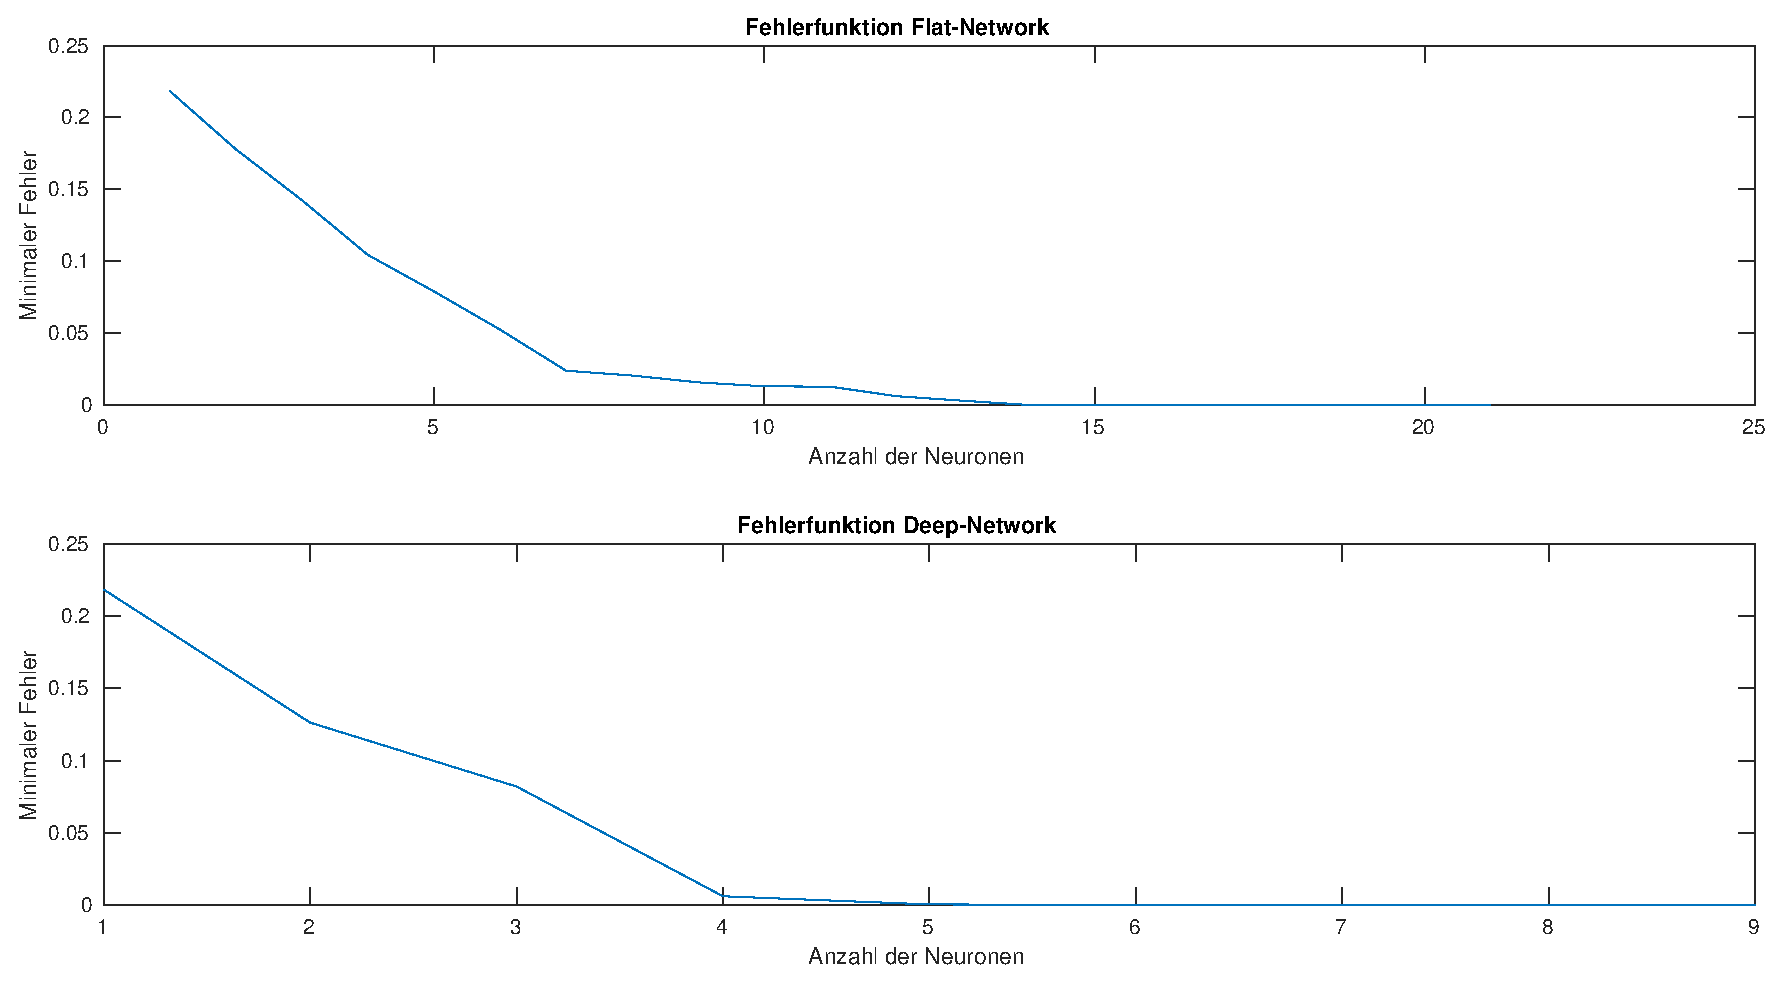
\includegraphics[width=\textwidth]{b07a02.eps}
                \caption{Verlauf der Fehlerfunktion}
            \end{figure}
    \end{enumerate}
\end{document}
